%!TEX program = xelatex

\documentclass[11pt,titlepage]{report}
%!TEX root = main.tex

\usepackage[T1]{fontenc}
\usepackage{lmodern}
\usepackage[svgnames]{xcolor}
\usepackage{fontspec} % XeLaTeX required!
\usepackage{graphicx}
\usepackage{circuitikz}
\usepackage{tikz}
\usepackage{pifont}
\usepackage[some]{background}
\usepackage{xltxtra} 
\usepackage{setspace}
\usepackage[absolute]{textpos}
\usepackage[latin1]{inputenc}
\usepackage[english]{babel}
\usepackage{graphicx}
\usepackage{wrapfig}
\usepackage{fullpage}
\usepackage[margin=1in]{geometry}
\usepackage{float}
\usepackage{url}
\usepackage{multicol}
\usepackage{hyperref}
\usepackage{titlepic}
\usepackage{standalone}
\usepackage{siunitx}
\usepackage{booktabs}
\usepackage{amsmath}
\usepackage{unicode-math}
\usepackage{verbatim}
\usepackage{enumitem}
\usepackage{listings}
\usepackage{multirow}
\usepackage{pgfplots}
\pgfplotsset{compat=1.8}
\usepackage{caption} 
\usepackage[parfill]{parskip}
\usepackage{import}
\usepackage[backend=bibtexu,texencoding=utf8,bibencoding=utf8,style=ieee,sortlocale=en_GB,language=auto]{biblatex}
\usepackage[strict,autostyle]{csquotes}
\usepackage[final]{pdfpages}
\usepackage{subcaption}
\usepackage{ifplatform}
%\captionsetup[table]{skip=10pt}


% Fix for includepdf bug in Mac OS X
\newcommand{\insertpdfpath}[1]{
	\ifwindows
	\newcommand{\insertpdf}[2]{\includepdf[pages=##1]{##2}}
	\else
	\newcommand{\insertpdf}[2]{\includepdf[pages=##1]{#1/##2}}
	\fi
}

%set fonts
\setmainfont[Ligatures=TeX]{Myriad Pro}
\setmathfont{Asana Math}
\setmonofont{Lucida Console}

\usepackage{titlesec, color}
\renewcommand{\familydefault}{\sfdefault} %set font family
\renewcommand{\arraystretch}{1.2} %set table vertical spacing
\setlength\parindent{0pt} %no paragraph indent
\hypersetup{ %setup hyperlinks
    colorlinks,
    citecolor=black,
    filecolor=black,
    linkcolor=black,
    urlcolor=black
}

%redesign chapter headings
\definecolor{gray75}{gray}{0.75}
\newcommand{\chapternumber}{\thechapter}
\newcommand{\hsp}{\hspace{20pt}}
\titleformat{\chapter}[hang]{\Huge\bfseries}{\chapternumber\hsp\textcolor{gray75}{|}\hsp}{0pt}{\Huge\bfseries}

%Redefine appendix headers
\renewcommand{\appendixname}{Appendix}
\renewcommand{\appendixtocname}{Appendices}
\renewcommand{\appendixpagename}{Appendices}

%For code listings
\definecolor{black}{rgb}{0,0,0}
\definecolor{browntags}{rgb}{0.65,0.1,0.1}
\definecolor{bluestrings}{rgb}{0,0,1}
\definecolor{graycomments}{rgb}{0.4,0.4,0.4}
\definecolor{redkeywords}{rgb}{1,0,0}
\definecolor{bluekeywords}{rgb}{0.13,0.13,0.8}
\definecolor{greencomments}{rgb}{0,0.5,0}
\definecolor{redstrings}{rgb}{0.9,0,0}
\definecolor{purpleidentifiers}{rgb}{0.01,0,0.01}


\lstdefinestyle{csharp}{
language=[Sharp]C,
showspaces=false,
showtabs=false,
breaklines=true,
showstringspaces=false,
breakatwhitespace=true,
escapeinside={(*@}{@*)},
columns=fullflexible,
commentstyle=\color{greencomments},
keywordstyle=\color{bluekeywords}\bfseries,
stringstyle=\color{redstrings},
identifierstyle=\color{purpleidentifiers},
basicstyle=\ttfamily\small}

\lstdefinestyle{c}{
language=C,
showspaces=false,
showtabs=false,
breaklines=true,
showstringspaces=false,
breakatwhitespace=true,
escapeinside={(*@}{@*)},
columns=fullflexible,
commentstyle=\color{greencomments},
keywordstyle=\color{bluekeywords}\bfseries,
stringstyle=\color{redstrings},
identifierstyle=\color{purpleidentifiers},
}

\lstdefinestyle{matlab}{
language=Matlab,
showspaces=false,
showtabs=false,
breaklines=true,
showstringspaces=false,
breakatwhitespace=true,
escapeinside={(*@}{@*)},
columns=fullflexible,
commentstyle=\color{greencomments},
keywordstyle=\color{bluekeywords}\bfseries,
stringstyle=\color{redstrings},
identifierstyle=\color{purpleidentifiers}
}

\lstdefinestyle{vhdl}{
language=VHDL,
showspaces=false,
showtabs=false,
breaklines=true,
showstringspaces=false,
breakatwhitespace=true,
escapeinside={(*@}{@*)},
columns=fullflexible,
commentstyle=\color{greencomments},
keywordstyle=\color{bluekeywords}\bfseries,
stringstyle=\color{redstrings},
identifierstyle=\color{purpleidentifiers}
}

\lstdefinestyle{xaml}{
language=XML,
showspaces=false,
showtabs=false,
breaklines=true,
showstringspaces=false,
breakatwhitespace=true,
escapeinside={(*@}{@*)},
columns=fullflexible,
commentstyle=\color{greencomments},
keywordstyle=\color{redkeywords},
stringstyle=\color{bluestrings},
tagstyle=\color{browntags},
morestring=[b]",
  morecomment=[s]{<?}{?>},
  morekeywords={xmlns,version,typex:AsyncRecords,x:Arguments,x:Boolean,x:Byte,x:Char,x:Class,x:ClassAttributes,x:ClassModifier,x:Code,x:ConnectionId,x:Decimal,x:Double,x:FactoryMethod,x:FieldModifier,x:Int16,x:Int32,x:Int64,x:Key,x:Members,x:Name,x:Object,x:Property,x:Shared,x:Single,x:String,x:Subclass,x:SynchronousMode,x:TimeSpan,x:TypeArguments,x:Uid,x:Uri,x:XData,Grid.Column,Grid.ColumnSpan,Click,ClipToBounds,Content,DropDownOpened,FontSize,Foreground,Header,Height,HorizontalAlignment,HorizontalContentAlignment,IsCancel,IsDefault,IsEnabled,IsSelected,Margin,MinHeight,MinWidth,Padding,SnapsToDevicePixels,Target,TextWrapping,Title,VerticalAlignment,VerticalContentAlignment,Width,WindowStartupLocation,Binding,Mode,OneWay,xmlns:x}
}

\lstdefinestyle{matlab}{
language=Matlab,
showspaces=false,
showtabs=false,
breaklines=true,
showstringspaces=false,
breakatwhitespace=true,
escapeinside={(*@}{@*)},
columns=fullflexible,
commentstyle=\color{greencomments},
keywordstyle=\color{bluekeywords}\bfseries,
stringstyle=\color{purpleidentifiers},
identifierstyle=\color{purpleidentifiers}
}

%defaults
\lstset{
basicstyle=\ttfamily\small,
extendedchars=false,
numbers=left,
numberstyle=\ttfamily\tiny,
stepnumber=1,
tabsize=4,
numbersep=5pt
}
\addbibresource{../../library/bibliography.bib}

\begin{document}

\chapter{Assignment 2}
\section{Observer design}
To have full state knowledge required for control, we designed an observer. This observer has to converge as fast as possible to the observed state. However, the fact that we can only observe approximately once per \SI{300}{ms}, puts constraints on the observer feedback matrix $\mat{L}$. We decided that the performance of a chosen feedback matrix $\mat{L}$ is given by

\begin{equation} \label{eq:ass-2-mse}
	\sum_{i=0}^{\infty} (\hat{\vec{y}_i}-\vec{y}_i)^2.
\end{equation}

Here the output of the observer at specified time $t$ with corresponding sample number $i$ is denoted by $\hat{\vec{y}_i}$ and the output measured, which is in our case the distance measured, by $\vec{y}_i$. Equation \ref{eq:ass-2-mse} is in fact the mean square error (MSE). Defining such a measure for performance allowed us to try many different eigenvalues for matrix $\mat{L}$ and observe the results. The results are shown in Figure~\ref{fig:ass-2-eigs}.

\begin{figure}[H]
	\begin{center}
		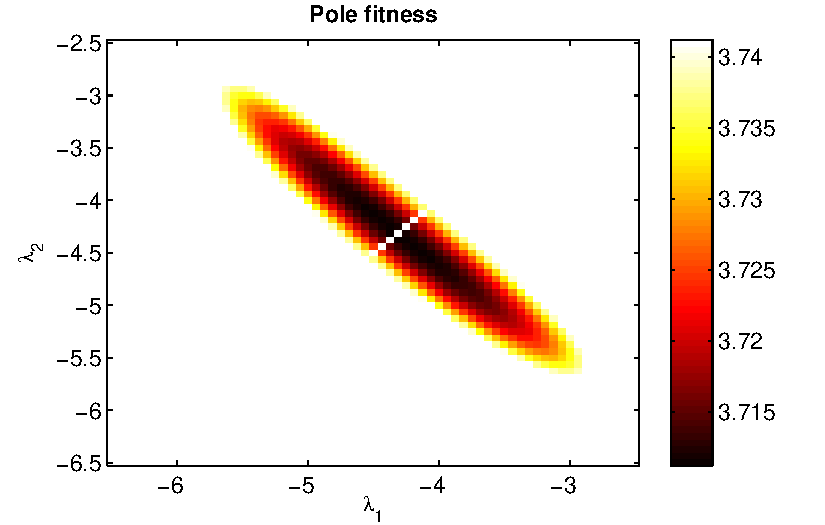
\includegraphics[width=.7\linewidth]{resource/pole-fitness.pdf}
	\end{center}
	\caption{Performance of the eigenvalues of matrix $\mat{L}$, darker is better}
	\label{fig:ass-2-eigs}
\end{figure}

There is one thing worth mentioning about the results shown in Figure~\ref{fig:ass-2-eigs}. The eigenvalues seem to converge to approximately $(-4.5,-4.5)$, but when they come very close to this value, they fail to perform. The ideal observer would converge critically damped. However, in the case of critically damped behaviour, $\lambda_1 = \lambda_2$, which is why they converge to a point $(a,a)$. Having said that, two eigenvalues of the same value render $\mat{A}$ undiagonalizable, which is why they seem to fail to perform. Critically damped behaviour is further explained in Section \ref{sec:ass-2-behav}.

One would think, that having poles with a real part as negative as possible, would result in the lowest convergence time. In the case of a continuous time space this would be true. However, we can only sample once in a while. Therefore, poles with a real part as negative as possible would very likely result in severe overshoot.

\section{Oscillatory and critically damped response}
\label{sec:ass-2-behav}
The response consists of two exponential functions, whose exponents are the eigenvalues. Therefore, to achieve an oscillatory response, the eigenvalues must be complex conjugated.

The situation is somewhat more complex regarding a perfect critically damped response. The solution of a state-space model is dependent of $e^{\mat{A} t}$, which can be written as

\begin{equation}
	e^{\mat{A} t} = \sum_{k=0}^{\infty} \frac{\mat{A}^k t^k}{k!}.
\end{equation}

If $\mat{A}$ is diagonalizable, then

\begin{equation} \label{eq:ass-2-matrix}
	e^{\mat{A} t} = P \begin{bmatrix}
		e^{\lambda_1 t} & 0 & & 0 \\
		0 & e^{\lambda_2 t} & & \\
		 & & \ddots & 0 \\
		 0 & & 0 & e^{\lambda_n t}
	\end{bmatrix} P^{-1}.
\end{equation}

The exponential functions in Equation \ref{eq:ass-2-matrix} show that this calculation yields us an overdamped response. We can therefore roughly state that, if $\mat{A}$ is diagonalizable, this corresponds with an overdamped response.

$e^{\mat{A} t}$ can also be calculated using the $\mat{A}$'s Jordan form. If $e^{\mat{A} t}$ is diagonalizable, then this Jordan form reduces to a regular diagonalization. However, if $e^{\mat{A} t}$ is not diagonalizable, then calculating $e^{\mat{A} t}$ using $\mat{A}$'s Jordan form turns out to give us a critically damped solution \cite{jordan-solution}. Therefore, if we were able to choose a feedback which would render $\mat{A} - \mat{B} \mat{K}$ not diagonalizable, then we would find a critically damped response.

Let us consider the case of a matrix $\mat{A} \in \mathbb{M}_{22}$. If $\lambda$ was to be an eigenvalue, then solving $\operatorname{null}{(\mat{A} - \lambda \mat{I})}$ would yield the corresponding eigenvectors. In general, $\operatorname{nullity}{(\mat{M})} + \operatorname{rank}{(\mat{M})} = n$. Therefore, in our case, $2 - \operatorname{rank}{(\mat{A} - \lambda \mat{I})} = \operatorname{nullity}{(\mat{A} - \lambda \mat{I})}$. However, if $\operatorname{rank}{(\mat{A} - \lambda \mat{I})} \ge 1$, which is the case if $\mat{A} - \lambda \mat{I} \neq \vec{0}$, then the dimension of the eigenspace corresponding with $\lambda$ can not equal two. Therefore, if $\lambda$ would have algebraic multiplicity two, then $\mat{A}$ would be not diagonalizable.

Combining the facts that \textbf{(1)} having a algebraic multiplicity of two renders $\mat{A}$ not diagonalizable, and \textbf{(2)} $\mat{A}$ not being diagonalizble leads us to a critically damped response, tempts us to argue that choosing two eigenvalues $\lambda_1$ and $\lambda_2$ with $|\lambda_1- \lambda_2|$ minimal, allows us to mimic an eigenvalue with algebraic multiplicity of two and consequently approximate critically damped behaviour. 

\section{Controlling the output}
Consider the state-space model

\begin{align}
	\dot{\vec{x}} &= \mat{A}\vec{x} + \mat{B}\vec{u}, \\
	\vec{y} &= \mat{C} \vec{x}. \label{eq:ass-2-model-output}
\end{align}

Let

\begin{equation}
	\vec{u} = -\mat{K}\vec{x} + \vec{r}
\end{equation}

be a feedback law which renders the considered state-space system asymptotically stable. Substituting $\vec{u}$ yields

\begin{equation} \label{eq:ass-2-derivative}
	\dot{\vec{x}} = (\mat{A} - \mat{B} \mat{K}) \vec{x} + \mat{B} \vec{r}.
\end{equation}

Using the fact that our system is asymptotically stable, we can argue that $\dot{\vec{x}} \to 0$ when $t \to \infty$. Combining Equation~\ref{eq:ass-2-model-output} and \ref{eq:ass-2-derivative} yields

\begin{equation}
	\vec{y} \to \mat{C} (\mat{B} \mat{K} - \mat{A})^{-1} \mat{B} \vec{r} \text{ when } t \to \infty.
\end{equation}

Therefore, the output $\vec{y}$ converges to the scaled applied input $\vec{r}$. We can utilize this fact to control the output of the model.

\section{Controller design}
Putting together the compensator, observer and output reference leaves us at the controller given by

\begin{align}
	\dot{\hat{\vec{x}}} &= (\mat{A}-\mat{L}\mat{C}-\mat{B}\mat{K}) \hat{\vec{x}} + \mat{B}(\mat{C}(\mat{B} \mat{K} - \mat{A})^{-1} \mat{B})^{-1} \vec{r} + \mat{L} \vec{y}, \\
	\vec{x} &= (\mat{C}(\mat{B} \mat{K} - \mat{A})^{-1} \mat{B})^{-1} \vec{r} - \mat{K} \hat{\vec{x}}.
\end{align}

Here the drive excitation is denoted by $\vec{x}$ and distance measured by $\vec{y}$. However, we can only regulate the throttle of KITT approximately once per \SI{300}{ms}. We must therefore discretize the controller. Discretization using Heun's method \cite{wikipedia-heuns} yields

\begin{align}
	f(\vec{x},\vec{r},\vec{y}) &= (\mat{A}-\mat{L}\mat{C}-\mat{B}\mat{K}) \hat{\vec{x}} + \mat{B}(\mat{C}(\mat{B} \mat{K} - \mat{A})^{-1} \mat{B})^{-1} \vec{r} + \mat{L} \vec{y}, \\
	\hat{\vec{x}}_n &= \hat{\vec{x}}_{n-1} + \frac{T}{2} \left( f\left(\vec{x}_{n-1},\vec{r}_{n-1},\vec{y}_{n-1} \right) + f\left( \vec{x}_{n-1} + T f(\vec{x}_{n-1},\vec{r}_{n-1},\vec{y}_{n-1}),\vec{r}_{n},\vec{y}_{n}\right) \right), \\
	\vec{x}_n &= (\mat{C}(\mat{B} \mat{K} - \mat{A})^{-1} \mat{B})^{-1} \vec{r}_n - \mat{K} \hat{\vec{x}}_n.
\end{align}

Heun's method averages the slopes at points $n$ and $n+1$ using Euler's method to predict the value at point $n+1$. This gives us a decent and relatively easy way to implement the approximation.

\begin{figure}[H]
	\begin{center}
		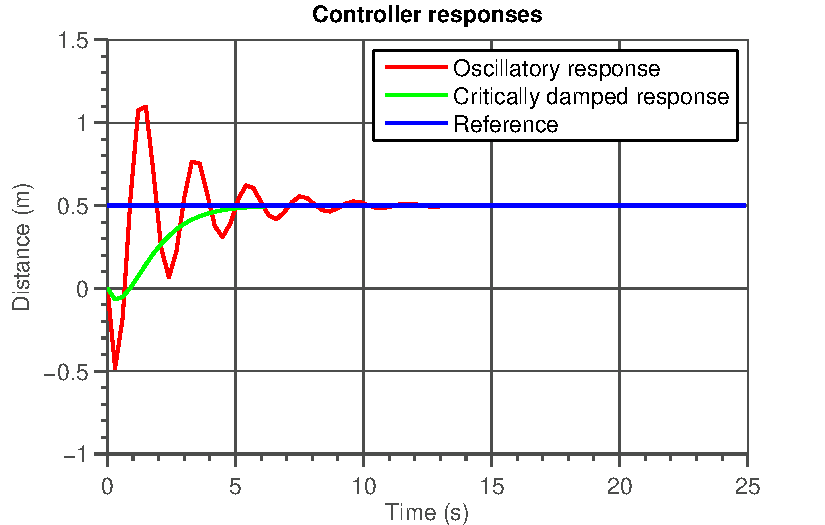
\includegraphics[width=0.7\linewidth]{resource/controller.pdf}
	\end{center}
	\caption{Oscillatory and critically damped response of the controller}
	\label{fig:ass-2-controller-response}
\end{figure}

Figure \ref{fig:ass-2-controller-response} shows two different responses of the controller. Both an oscillatory and critically damped behaviour is shown. We can see that the controller converges the model to the specified reference. There is, however, something to notice. Both responses first tend to diverge from the reference. This is because the system is non-minimum phase.

\section{Controlling KITT}
Implementing the controller was not as straightforward as conceived. Here we present difficulties faced during the implementation.
\begin{itemize}
	\item The excitation of car to the specified PWM signal is heavily influenced by the battery voltage.
	\item The speed of the car is discretized; we can only send an integer drive value to KITT. This raised the problem that KITT would not drive for a signal lower than a certain value, which caused a steady-state error with respect to the reference distance.
	\item The fitted model only approximates the real situation.
	\item The sampling time would sometimes turn out unacceptably high, up to \SI{600}{ms}. This high latency caused, in combination with the minimum driving speed of KITT, an inevitable oscillatory response. \texttt{MATLAB}'s serial toolkit turned out to be the cause of this lag. Eventually we want to implement the communication in our C\# environment, so this problem should resolve itself.
	\item Although we applied our designed filters, the sensors would sometimes provide incorrect values.
\end{itemize}
Even though we encountered all these non-linearities, we were actually able to control the car up to some level. Keeping in mind all these non-linear aspects, the theory does, within some boundaries (i.e. the discussed non-linearities), match the reality. However, the responses measured do only to a certain extent match the simulated responses.

\begin{figure}[H]
	\begin{subfigure}{.5\textwidth}
		\centering
		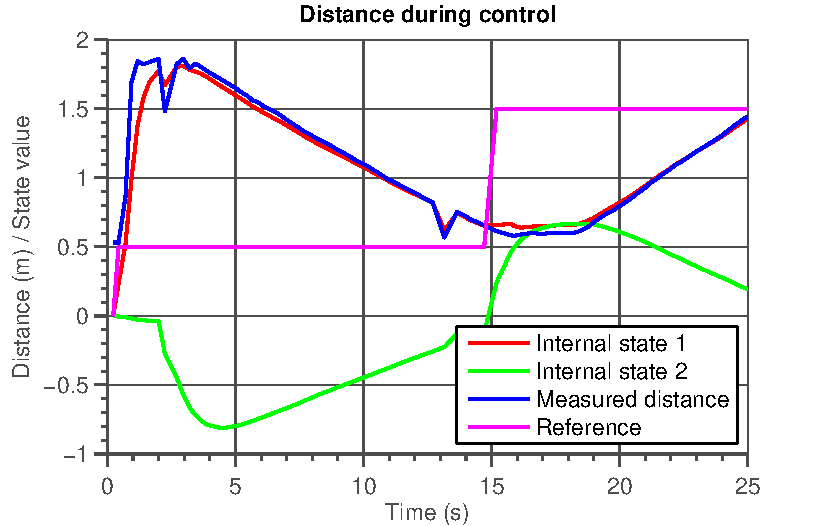
\includegraphics[width=\linewidth]{resource/measurement-states.pdf}
		\caption{Internal states, measured distance and reference during control}
	\end{subfigure}
	\begin{subfigure}{.5\textwidth}
		\centering
		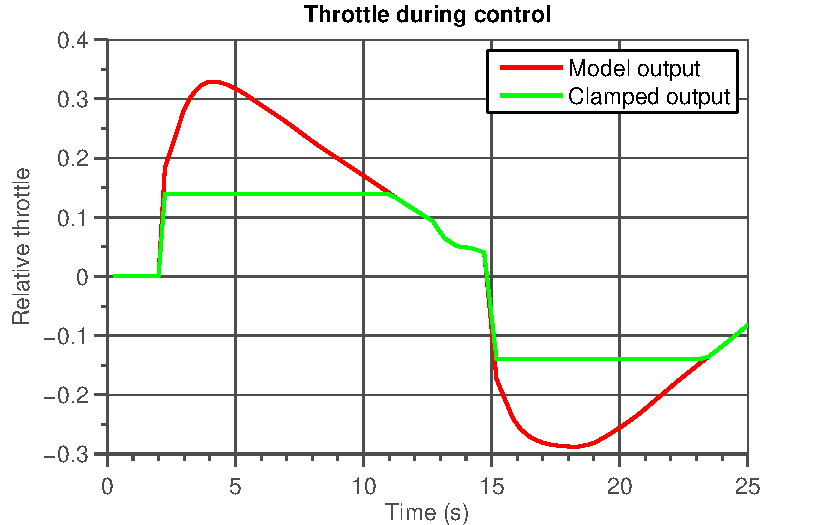
\includegraphics[width=\linewidth]{resource/measurement-drive.pdf}
		\caption{Relative throttle during control}
	\end{subfigure}
	\caption{Measurement results of KITT controlled by the designed controller}
	\label{fig:ass-2-kitt-controlled}
\end{figure}

Figure \ref{fig:ass-2-kitt-controlled} shows the results of KITT being controlled by the designed controller. One can see that the controller effectively drives KITT to the referenced distance. We have limited KITT's speed to prevent unwanted accidents.

\section{Controller revisited}
If we introduce the feedback law

\begin{equation}
	\vec{u} = -\mat{K}(\vec{x} - \vec{x}_{ref})
\end{equation}

and argue that $\dot{\vec{x}} \to 0$ when $t \to \infty$ then we obtain

\begin{equation} \label{eq:ass-2-rev}
	(\mat{B} \mat{K} - \mat{A}) \vec{x} = \mat{B} \mat{K} \vec{x}_{ref}.
\end{equation}

Let $\vec{x}$ and $\vec{x}_{ref}$ be of the form (snelheid is 2e item, die gaat naar 0 als t naar infty!)

\begin{equation}
	\vec{x} = \begin{bmatrix}
		d \\
		0
	\end{bmatrix},
	\vec{x}_{ref} = \begin{bmatrix}
		d_{ref} \\
		0
	\end{bmatrix}
\end{equation}

and $\mat{A}$ be of the form (specifiek ons model)

\begin{equation}
	\mat{A} = \begin{bmatrix}
		0 & a \\
		0 & b
	\end{bmatrix},
\end{equation}

then solving Equation \ref{eq:ass-2-rev} for $\vec{x}$ yields

\begin{equation}
	\vec{x} = \vec{x}_{ref}.
\end{equation}

\begin{align}
	\dot{\vec{x}} &= (\mat{A} - \mat{B} \mat{K}) \vec{x} + \mat{B} \mat{K} \vec{x}_{ref}, \\
	\vec{y} &= \mat{C} \vec{x}
\end{align}


\end{document}